\subsection{Misclassifications}
\label{sec:predictions-misclassifications}
By comparing all misclassifications of all networks several similarities are found.
It is noticed that an object with a wrong prediction is likely to reappear across different networks.
Not always with the exact same material, though, but this could be due to different weight initializations.
Some examples are shown in \figref{fig:small-features}.
The most common reason for predicting the wrong color class within the same object category class are small color marks.
\begin{figure}
	\centering
	\begin{subfigure}{.3\textwidth}
		\centering
		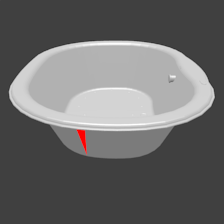
\includegraphics[width=.8\textwidth]{images/bathtub_0117_2_006.png}
		\caption{Predicted as blank}
		\label{fig:small-features-a}
	\end{subfigure}
	%
	\begin{subfigure}{.3\textwidth}
		\centering
		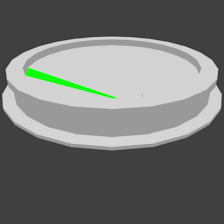
\includegraphics[width=.8\textwidth]{images/bathtub_0127_1_007.png}
		\caption{Predicted as green-red}
		\label{fig:small-features-b}
	\end{subfigure}
	%
	\begin{subfigure}{.3\textwidth}
		\centering
		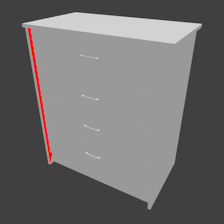
\includegraphics[width=.8\textwidth]{images/dresser_0215_2_010.png}
		\caption{Predicted as blank}
		\label{fig:small-features-c}
	\end{subfigure}
	
	\begin{subfigure}{.3\textwidth}
		\centering
		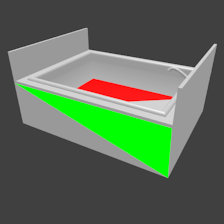
\includegraphics[width=.8\textwidth]{images/bathtub_0125_3_004.png}
		\caption{Predicted as green}
		\label{fig:small-features-d}
	\end{subfigure}
	%
	\begin{subfigure}{.3\textwidth}
		\centering
		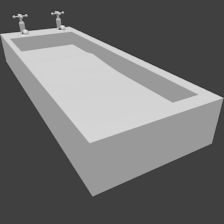
\includegraphics[width=.8\textwidth]{images/bathtub_0111_0_011.png}
		\caption{Predicted as blank sofa}
		\label{fig:small-features-e}
	\end{subfigure}
	%
	\begin{subfigure}{.3\textwidth}
		\centering
		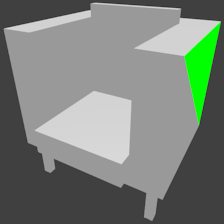
\includegraphics[width=.8\textwidth]{images/sofa_0681_1_010.png}
		\caption{Predicted as green-green dresser}
		\label{fig:small-features-f}
	\end{subfigure}
	\caption[Reasons for incorrect predictions]{Reasons for incorrect predictions are small features, hidden features, and missing shadows.}
	\label{fig:small-features}
\end{figure}
\figref{fig:small-features-a}, \figref{fig:small-features-b} and \figref{fig:small-features-c} show such views.
In this case the color class of an object related to the first is classified as blank, the one to the second as green-red and the one to the third as blank.
Why the material color is predicted wrong, however, remains unknown.
For the view in \figref{fig:small-features-d} the red face is never seen completely in its multi-view, hence, it is never seen in a triangular shape like usual faces except for one view.
There it is truncated to a small triangular, though, and experiences the same problems as the preceding views presumably.
Two optimal faces next to each other forming a rectangle result in a correct classification in general, though.
The case of two faces building a larger triangle is not present in the dataset.
Although it is assumed that such a multi-view would be predicted wrong.
The reason for predicting bathtubs incorrectly as sofas like in \figref{fig:small-features-e} are mostly missing shadows.
Because mainly the long left side transitions into the horizontal plane due to a missing sharp shadow at the edge the actual bathtub is more likely to be predicted as a sofa.
This object is indeed likely to reappear in different networks as a wrong prediction.
However, the actual and predicted color class differs.
\figref{fig:small-features-f} is classified as a dresser with a green-green color mark.
Though, it is a sofa and has only one green material feature.
This shows that many objects are just predicted wrong without an interpretable or obvious cause.